\section{Splinter}

\subsection{Motivation}
Many online services let users query large public datasets:
some examples include restaurant sites, product catalogs, stock quotes,
and searching for directions on maps. In these services, 
any user can query the data, and the datasets themselves
are not sensitive. However, web services can infer a great deal of identifiable and sensitive
user information from these queries, such as her current location,
political affiliation, sexual orientation, income, etc.~\cite{narayanan2010myths, narayanan2008robust}.
Web services can use this information maliciously and put users at risk to practices such as
discriminatory pricing~\cite{amazon-disc-pricing, price-disc2, hannak2014measuring}.
For example, online stores have charged users different prices based on location~\cite{price-disc}, and
travel sites have also increased prices for certain frequently searched flights~\cite{travel-pricing}.
Even when the services are honest, server compromise and subpoenas can leak the sensitive user
information on these services~\cite{ravichandran2009capturing, yelp-compromise, twitter-compromise}.

This thesis presents Splinter, a system that protects users' queries on public datasets
while achieving practical performance for many current web applications.
In Splinter, the user divides each query into shares and sends them to different
\emph{providers}, which are services hosting a copy of the dataset (Figure~\ref{fig:overview}).
As long as any one of the providers is honest and does not
collude with the others, the providers cannot discover sensitive
information in the query.
However, given responses from all the providers, the user
can compute the answer to her query.

\begin{figure}
	\centering
	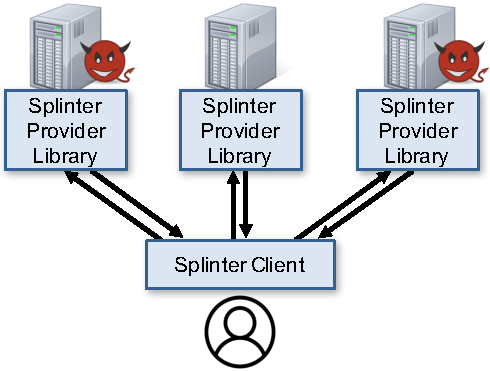
\includegraphics{splinter-overview.pdf}
	\caption{
		Splinter architecture. 
		The Splinter client splits each user query into shares and sends them to multiple
		providers. It then combines their results to obtain
		the final answer.
		The user's query remains private as long as any one provider is honest.
	}
	\label{fig:overview}
\end{figure}

Previous private query systems have generally not achieved practical performance
because they use expensive cryptographic primitives and protocols.
For example, systems based on Private Information Retrieval (PIR)~\cite{goldberg,chor1997private,pir-search} require many round trips and high bandwidth for complex queries, while systems based on garbled
circuits~\cite{wu2016,lan2016embark,ben2008fairplaymp} have a high computational cost.
These approaches are especially costly for mobile clients on high-latency networks.

Instead, Splinter uses and extends a recent cryptographic primitive called
Function Secret Sharing (FSS)~\cite{fss, gilboa2014distributed}, which makes it up to an
order of magnitude faster than prior systems.
FSS allows the client to split certain functions into shares that keep parameters of the
function hidden unless all the providers collude.
With judicious use of FSS, many queries can be answered at low CPU and bandwidth cost in only a single network round trip.

Splinter makes two contributions over previous work on FSS.
First, prior work has only demonstrated efficient FSS protocols for point and interval functions with additive aggregates such as SUMs~\cite{fss}.
We present protocols that support a more complex set of non-additive aggregates such as MAX/MIN and TOPK at low computational and communication cost.
Together, these protocols let Splinter support a subset of SQL that can capture many popular online applications.

Second, we develop an optimized implementation of FSS for modern hardware that leverages AES-NI~\cite{aes-ni} instructions and multicore CPUs.
For example, using the one-way compression functions that utilize modern AES instruction sets, our implementation is 2.5$\times$ faster per core than a na\"ive implementation of FSS.
Together, these optimizations let Splinter query datasets with millions of records at sub-second latency on a single server.

We evaluate Splinter by implementing 
three applications over it: a restaurant review site similar to Yelp, 
airline ticket search, and map routing.
For all of our applications, Splinter can execute queries in less than 1.6 seconds, at a cost of less than $0.02\cent$ in server resources on Amazon EC2.
Splinter's low cost means that providers could profitably run a Splinter-based service
similar to OpenStreetMap routing~\cite{osm}, an open-source maps service, while only charging users a few dollars per month.

Splinter aims to protect sensitive information in users' queries
from providers. This section provides an overview of Splinter's architecture,
security goals, and threat model.

\subsection{Splinter Overview}
\label{sec:model}
There are two main principals in Splinter: the \emph{user} and the \emph{providers}.
Each provider hosts a copy of the data. Providers can 
retrieve this data from a public repository or mirror site.
For example, OpenStreetMap~\cite{osm} publishes publicly available 
map, point-of-interest, and traffic data. 
For a given user query, all the providers have to run it on the same
view of the data. Maintaining data consistency
from mirror sites is beyond the scope of this thesis, but
standard techniques can be used~\cite{tewari2002wcdp,chi2008novel}.

As shown in Figure~\ref{fig:overview}, 
to issue a query in Splinter, a user
splits her query into \textit{shares}, using the Splinter client,
and submits each share to a different provider.
The user can select any providers of her choice that host the dataset.
The providers use their shares to execute the user's query 
over the cleartext public data, using the Splinter provider library. 
As long as one provider is \textit{honest}
(does not collude with others), the user's sensitive information in the original query
remains private. When the user receives the responses from the providers,
she combines them to obtain the final answer to her original query. 
%In Section~\ref{sec:queries},
%we will describe in more detail how the user creates these function shares and how
%the provider uses them to execute the user's query.

\subsection{Security Goals}
\label{sec:query_model}
The goal of Splinter is to hide sensitive parameters in
a user's query.
Specifically, Splinter lets users run \emph{parametrized queries}, 
where both the parameters and query results are hidden from providers.
For example, consider the following query, which finds the 10 cheapest flights between a source and destination:
\begin{verbatim}
SELECT TOP 10 flightid FROM flights
WHERE source = ? AND dest = ? 
ORDER BY price
\end{verbatim}
Splinter hides the information represented by the questions marks, i.e.,
the source and destination in this example.
The column names being selected and filtered are not hidden.
Finally, Splinter also hides the query's results---otherwise,
these might be used to infer the source and destination. 
Splinter supports a subset of the SQL language.

The easiest way to achieve this property would be for users to download the whole database
and run the queries locally.
However, this requires substantial bandwidth and computation for the user.
Moreover, many datasets change constantly, e.g., to include traffic information or new product reviews.
It would be impractical for the user to continuously download these updates.
Therefore, our performance objective is to minimize computation and communication costs.
For a database of $n$ records, Splinter only requires $O(n \log n)$ computation at the
providers and $O(\log n)$ communication.

\subsection{Threat Model}
Splinter keeps the parameters in the user's query hidden
as long as at least one of the user-chosen providers does not collude with others. 
Splinter also assumes these providers are \textit{honest but curious}: a provider can observe the interactions between
itself and the client, but 
Splinter does not protect against providers returning incorrect results or maliciously modifying the dataset.

We assume that the user communicates with each provider through a secure channel (e.g., using SSL),
and that the user's Splinter client is uncompromised. 
%Protecting attacks on a user's machine are outside of the scope of Splinter.
Our cryptographic assumptions are standard.
We only assume the existence of one-way functions in our two-provider implementation.
In our implementation for multiple providers, the security of Paillier encryption~\cite{paillier} is also assumed.
%the dec
